% ===================================
% CODICE LaTeX PER GRAFICI E TABELLE
% Tesi GDO - Capitoli 1 e 2
% ===================================
% filepath: c:\Users\saint\tesi\nuovi grafi 1 e 2.tex
\documentclass[border=10pt]{standalone}
% Pacchetti necessari
\usepackage[utf8]{inputenc}
\usepackage[T1]{fontenc}
\usepackage{amsmath}
\usepackage{amssymb}    
\usepackage{graphicx}
\usepackage{caption}
\usepackage{subcaption} % Per sottotitoli nelle figure
% Preambolo necessario:
\usepackage{tikz}
\usepackage{pgfplots}
\usepackage{booktabs}
\usepackage{multirow}
\pgfplotsset{compat=1.17}
\usetikzlibrary{pgfplots.polar}
\begin{document}
% FIGURA 2.3: Decomposizione STL
\centering
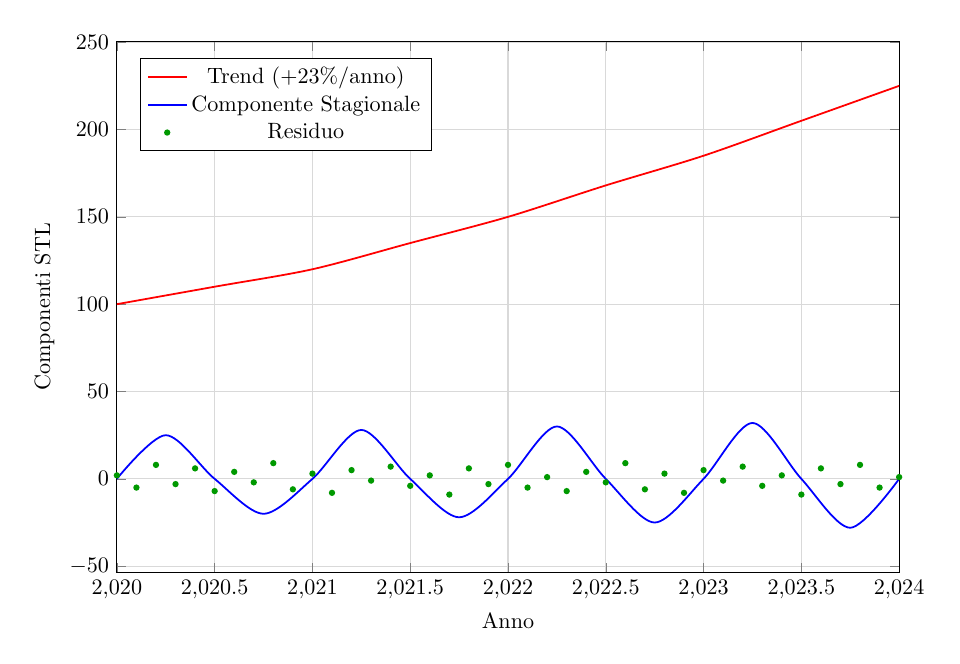
\begin{tikzpicture}[scale=0.8, transform shape]
\begin{axis}[
    width=14cm,
    height=10cm,
    xlabel={Anno},
    ylabel={Componenti STL},
    xmin=2020,
    xmax=2024,
    legend pos=north west,
    grid=major,
    grid style={line width=0.5pt, draw=gray!30}
]

% Trend
\addplot[thick,red,smooth] table[x=year,y=trend] {
year trend
2020.0 100
2020.5 110
2021.0 120
2021.5 135
2022.0 150
2022.5 168
2023.0 185
2023.5 205
2024.0 225
};
\addlegendentry{Trend (+23\%/anno)}

% Stagionalità
\addplot[thick,blue,smooth] table[x=year,y=seasonal] {
year seasonal
2020.0 0
2020.25 25
2020.5 0
2020.75 -20
2021.0 0
2021.25 28
2021.5 0
2021.75 -22
2022.0 0
2022.25 30
2022.5 0
2022.75 -25
2023.0 0
2023.25 32
2023.5 0
2023.75 -28
2024.0 0
};
\addlegendentry{Componente Stagionale}

% Residuo
\addplot[thick,green!60!black,only marks,mark size=1pt] table[x=year,y=residual] {
year residual
2020.0 2
2020.1 -5
2020.2 8
2020.3 -3
2020.4 6
2020.5 -7
2020.6 4
2020.7 -2
2020.8 9
2020.9 -6
2021.0 3
2021.1 -8
2021.2 5
2021.3 -1
2021.4 7
2021.5 -4
2021.6 2
2021.7 -9
2021.8 6
2021.9 -3
2022.0 8
2022.1 -5
2022.2 1
2022.3 -7
2022.4 4
2022.5 -2
2022.6 9
2022.7 -6
2022.8 3
2022.9 -8
2023.0 5
2023.1 -1
2023.2 7
2023.3 -4
2023.4 2
2023.5 -9
2023.6 6
2023.7 -3
2023.8 8
2023.9 -5
2024.0 1
};
\addlegendentry{Residuo}

\end{axis}
\end{tikzpicture}
\end{document}
